
\section*{Annexe 1 - Détail des éléments d'un des systèmes du VBB}
\begin{multicols}{2}
%\begin{figure}[!h]
%\centering
\begin{center}
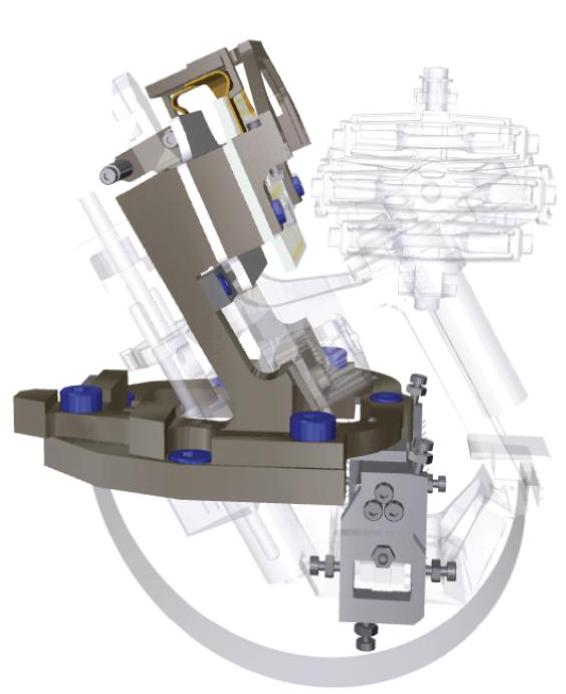
\includegraphics[height = 6.5cm]{2024_04_26_3285cfc264024262add0g-15(3)}
\captionof{figure}{\label{ccmp2023_fig_ann_1_1} Bâti (1)}
\end{center}
\begin{center}
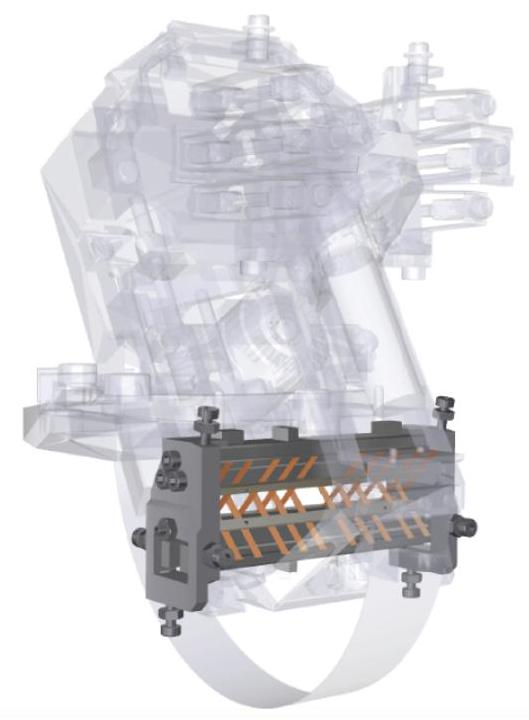
\includegraphics[height = 6.5cm]{2024_04_26_3285cfc264024262add0g-15(2)}
\captionof{figure}{\label{ccmp2023_fig_ann_1_2}Articulation à lamelles entre (1) et (2)}
\end{center}
\end{multicols}

\begin{multicols}{2}
%\begin{figure}[!h]
%\centering
\begin{center}
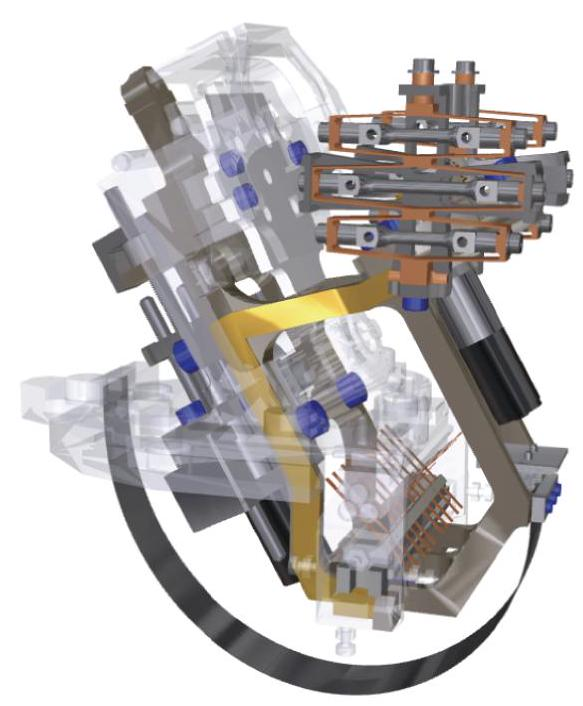
\includegraphics[height = 6.5cm]{2024_04_26_3285cfc264024262add0g-15}
\captionof{figure}{\label{ccmp2023_fig_ann_1_3}Pendule (2)}
\end{center}
\begin{center}
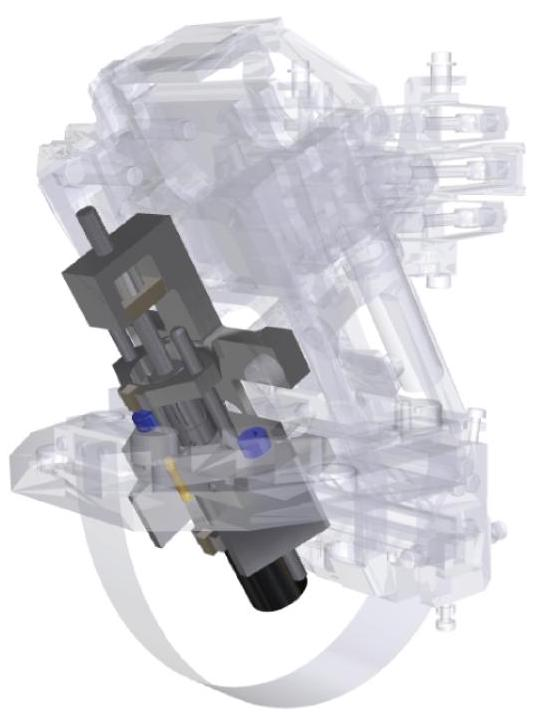
\includegraphics[height = 6.5cm]{2024_04_26_3285cfc264024262add0g-15(1)}
\captionof{figure}{\label{ccmp2023_fig_ann_1_4}Mécanisme de translation du centre d'inertie de (2)}
\end{center}
\end{multicols}
%
%
%
%\begin{figure}[!h]
%\centering
%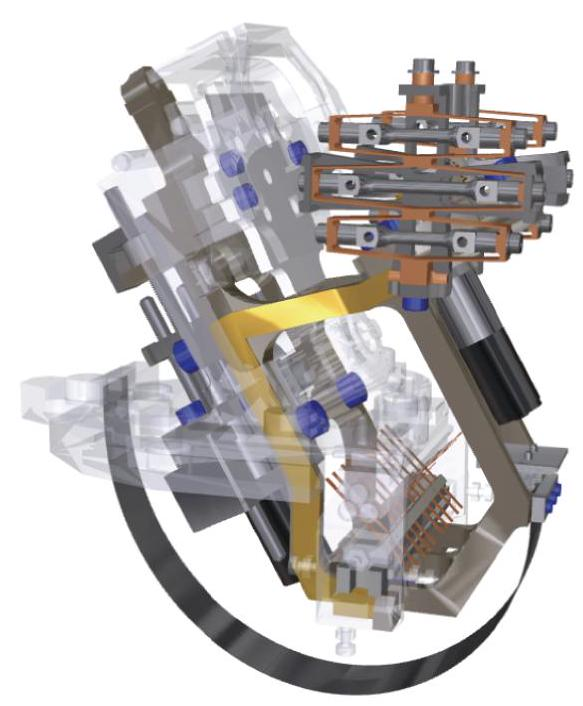
\includegraphics[width=.5\textwidth]{2024_04_26_3285cfc264024262add0g-15}
%\caption{\label{ccmp2023_ann_1_2} pendule (2)}
%\end{figure}
%
%
%
%\begin{figure}[!h]
%\centering
%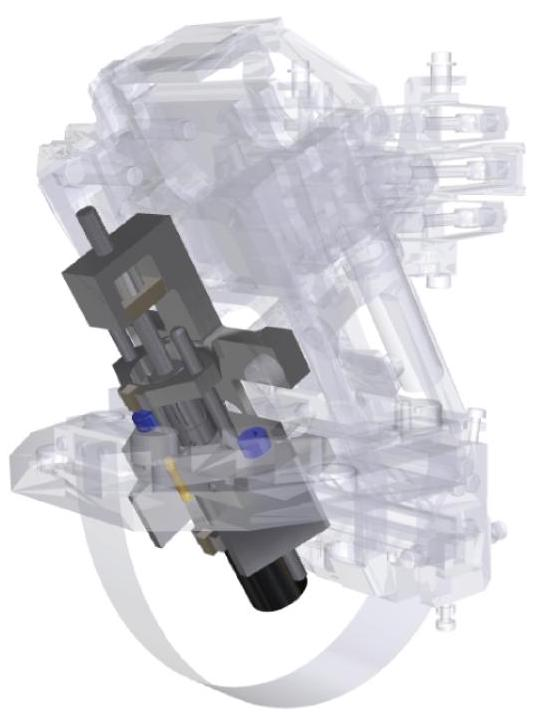
\includegraphics[width=.5\textwidth]{2024_04_26_3285cfc264024262add0g-15(1)}
%\caption{\label{ccmp2023_ann_1_3}mécanisme de translation du centre d'inertie de (2)}
%\end{figure}


%
%\section*{Annexe 2 - Modèle cinématique du système en l'absence de séisme}
%\begin{figure}[!h]
%\centering
%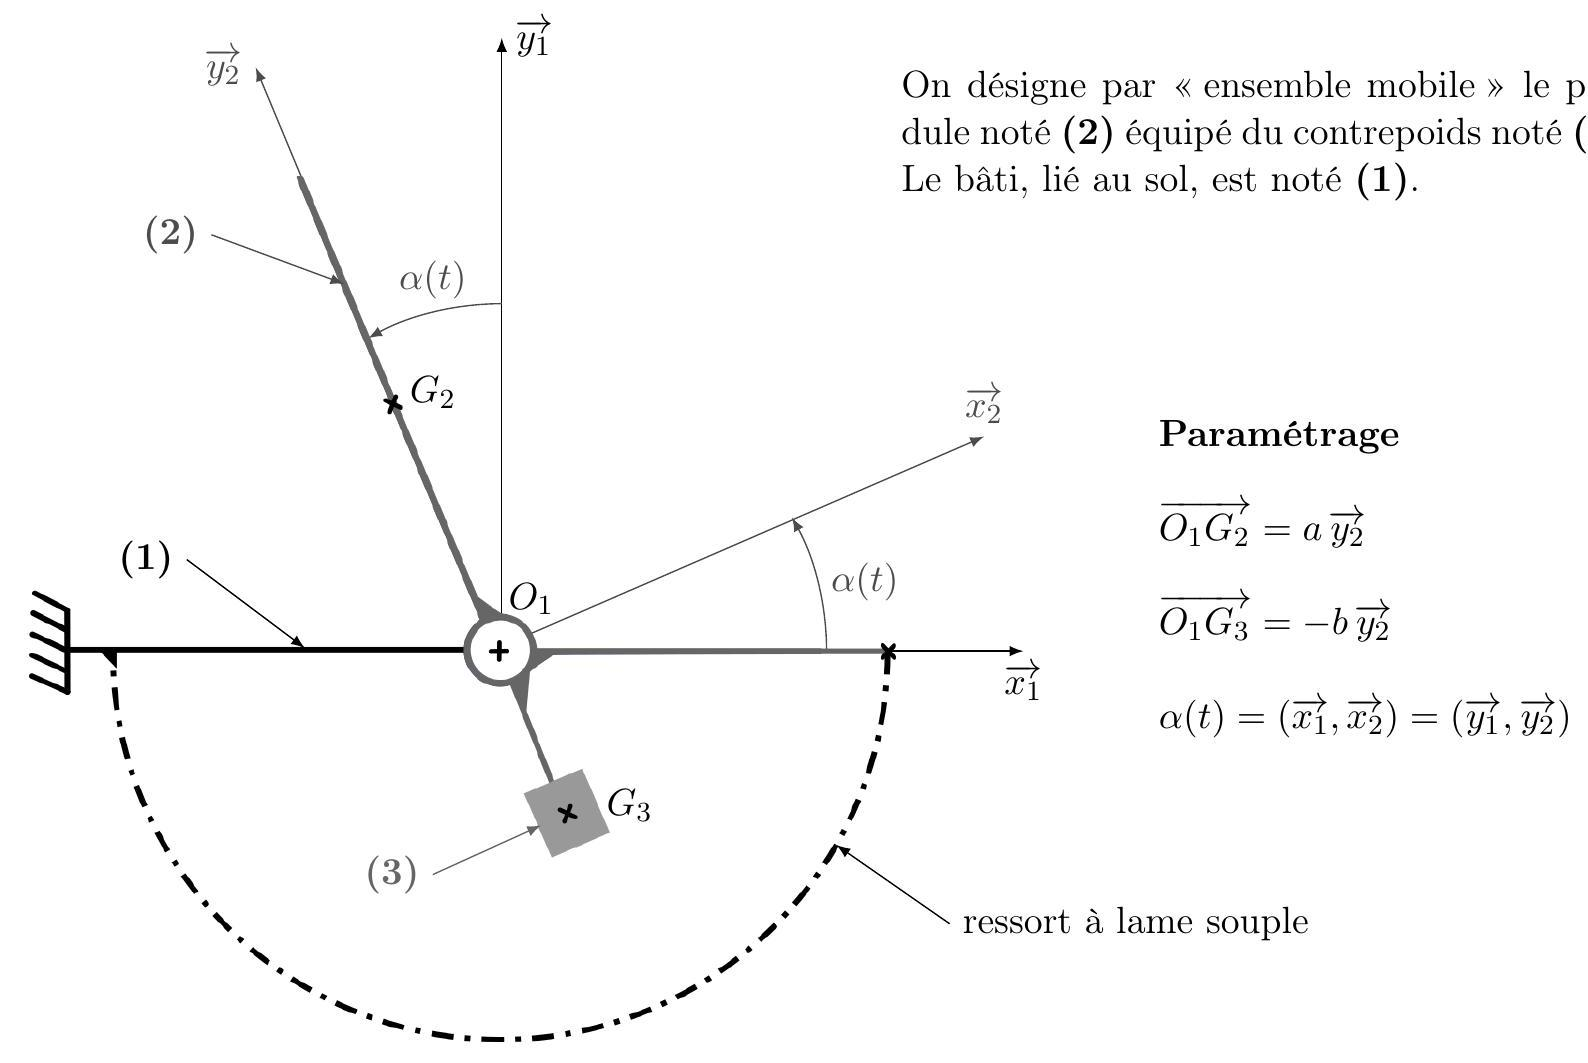
\includegraphics[width=\textwidth]{2024_04_26_3285cfc264024262add0g-16}
%%\caption{\label{ccmp2023_fig_01}}
%\end{figure}
%
%\section*{Notations}
%\begin{center}
%\begin{tabular}{|c|l|}
%\hline
%$G_{2}$ & centre d'inertie du pendule (2) \\
%\hline
%$M_{2}$ & masse du pendule (2) \\
%\hline
%$G_{3}$ & centre d'inertie du contrepoids (3) \\
%\hline
%$m_{3}$ & masse du contrepoids (3) \\
%\hline
%$C_{0}$ & \begin{tabular}{l}
%moment de précontrainte de l'ensemble \\
%\{ressort + articulation $\}$ sur $\{(\mathbf{2})+(\mathbf{3})\}$ \\
%\end{tabular} \\
%\hline
%$k$ & \begin{tabular}{l}
%raideur de l'ensemble \{ressort + articu- \\
%lation\} sur l'axe $\left(O_{1}, \overrightarrow{z_{1}}\right)$ \\
%\end{tabular} \\
%\hline
%$\alpha_{0}$ & \begin{tabular}{l}
%position angulaire à vide de l'ensemble \\
%mobile \\
%\end{tabular} \\
%\hline
%$\alpha_{\mathrm{eq}}$ & \begin{tabular}{l}
%position angulaire de l'ensemble mobile \\
%à l'équilibre (sous l'effet des actions de \\
%la pesanteur et du ressort) \\
%\end{tabular} \\
%\hline
%$g_{T}$ & \begin{tabular}{l}
%champ de pesanteur à la surface de la \\
%Terre, de direction $-\overrightarrow{y_{1}}$ \\
%\end{tabular} \\
%\hline
%$g_{M}$ & \begin{tabular}{l}
%champ de pesanteur à la surface de Mars, \\
%de direction $-\overrightarrow{y_{1}}$ \\
%\end{tabular} \\
%\hline
%\end{tabular}
%\end{center}
%
%\section*{Hypothèses}
%Le référentiel $\mathcal{R}_{1}$, auquel est associé le repère $R_{1}=\left(O_{1}, \overrightarrow{x_{1}}, \overrightarrow{y_{1}}, \overrightarrow{z_{1}}\right)$ lié au sol, est supposé galiléen en l'absence de séisme.
%
%La liaison pivot réalisée par l'articulation à lamelle sur l'axe de rotation $\left(O_{1}, \overrightarrow{z_{1}}\right)$ de l'ensemble mobile n'est pas parfaite. Les frottements visqueux sont pris en compte à travers un coefficient de frottement $\mu(\mu>0)$ :
%
%$$
%\left\{\mathcal{T}_{1 \rightarrow(2+3)}\right\}=\left\{\begin{array}{c}
%X_{O} \overrightarrow{x_{1}}+Y_{O} \overrightarrow{y_{1}}+Z_{O} \overrightarrow{z_{1}} \\
%L_{O} \overrightarrow{x_{1}}+M_{O} \overrightarrow{y_{1}}-\mu \dot{\alpha}(t) \overrightarrow{z_{1}}
%\end{array}\right\}_{O_{1}}
%$$
%
%L'action de rappel de l'ensemble $\{$ ressort + articulation $\}$ est assimilée à un couple pur sur l'axe de rotation $\left(O_{1}, \overrightarrow{z_{1}}\right)$ de l'ensemble mobile :
%
%$\left\{\mathcal{T}_{\text {ressort } \rightarrow(2+3)}\right\}=\left\{\begin{array}{c}\overrightarrow{0} \\ \left(C_{0}-k\left(\alpha(t)-\alpha_{0}\right)\right) \overrightarrow{z_{1}}\end{array}\right\}_{O_{1}}$
%
%Annexe 3 - Schéma cinématique du mécanisme de translation de la position du centre d'inertie du pendule
%
%\begin{figure}[!h]
%\centering
%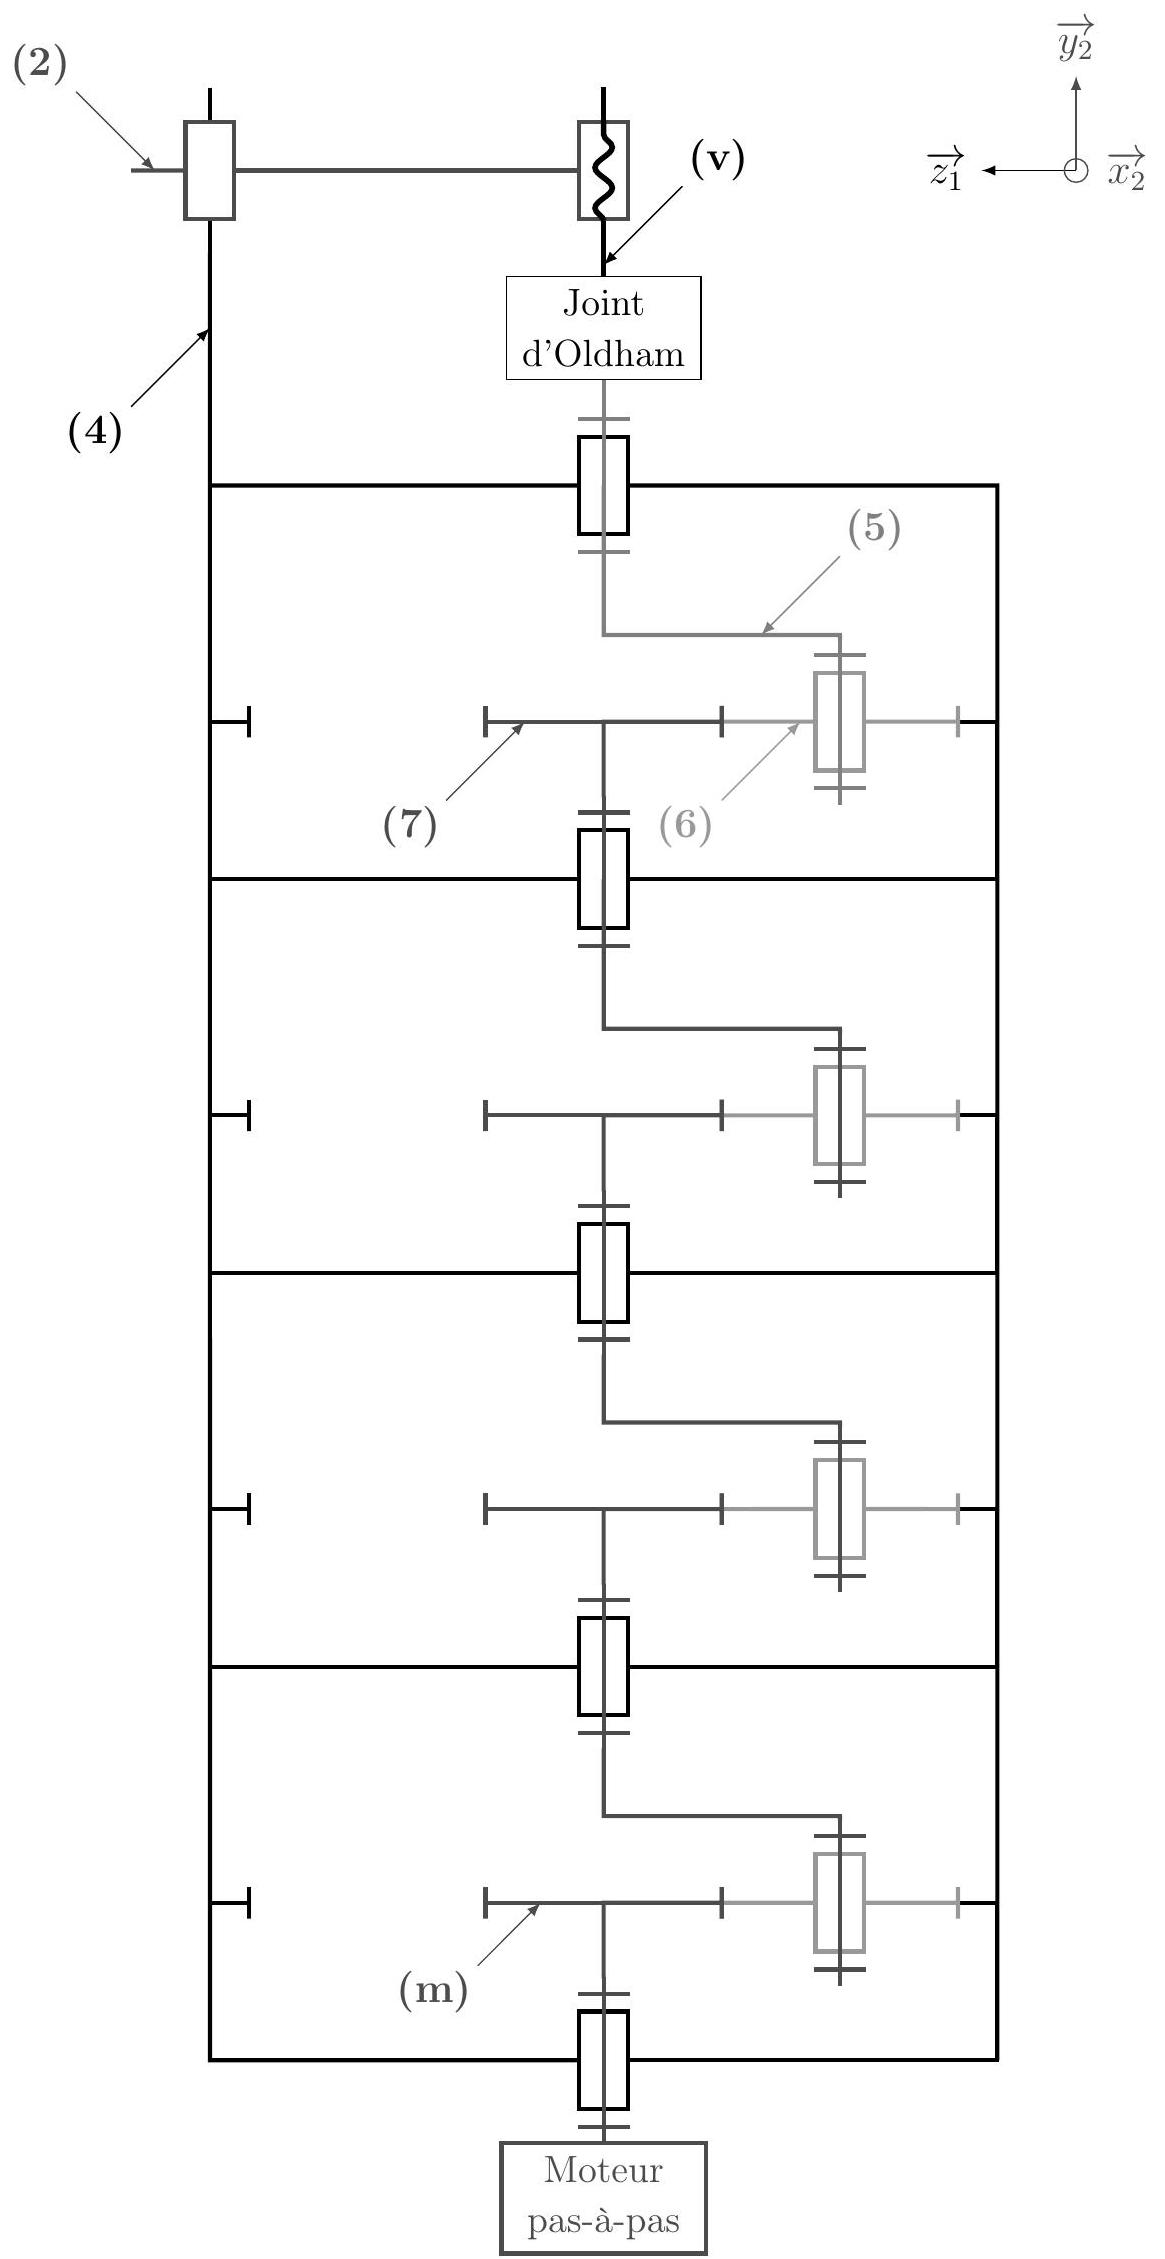
\includegraphics[width=\textwidth]{2024_04_26_3285cfc264024262add0g-17}
%%\caption{\label{ccmp2023_fig_01}
%\end{figure}
%
%%Page $3 / 5$
%
%\section*{Annexe 4 - Modèle cinématique du système lors d'un séisme}
%Les torseurs d'actions mécaniques et les notations de l'Annexe 2 restent valables.
%
%\begin{figure}[!h]
%\centering
%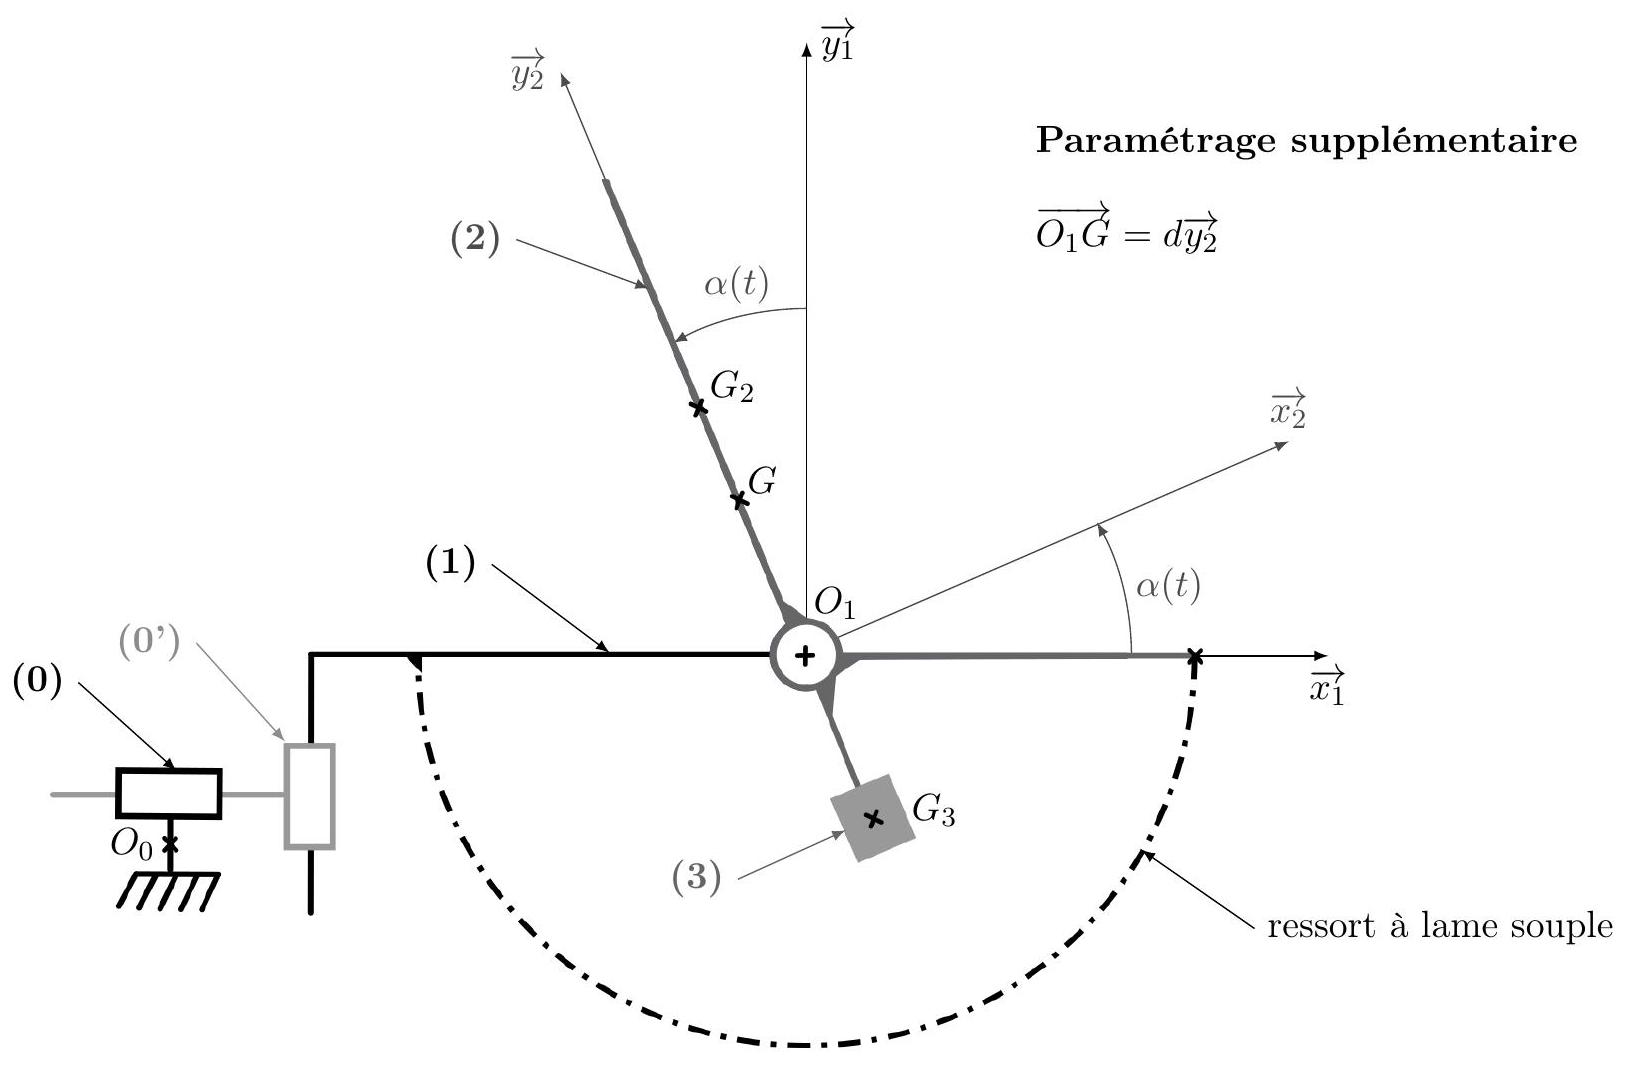
\includegraphics[width=\textwidth]{2024_04_26_3285cfc264024262add0g-18}
%%\caption{\label{ccmp2023_fig_01}
%\end{figure}
%
%Notations et hypothèses supplémentaires
%
%\begin{center}
%\begin{tabular}{|c|l|}
%\hline
%$G$ & \begin{tabular}{l}
%centre d'inertie de l'ensemble mobile \\
%$\{(\mathbf{2})+(\mathbf{3})\}$ testé sur Terre \\
%\end{tabular} \\
%\hline
%$M$ & masse de l'ensemble mobile $\{\mathbf{( 2 )}+\mathbf{( 3 )}\}$ \\
%\hline
%$I_{z z}$ & \begin{tabular}{l}
%moment d'inertie de l'ensemble mobile \\
%$\{(\mathbf{2})+(\mathbf{3})\}$ sur l'axe $\left(O_{1}, \overrightarrow{z_{1}}\right)$ \\
%\end{tabular} \\
%\hline
%\end{tabular}
%\end{center}
%
%Le référentiel $\mathcal{R}_{0}$, auquel est associé le repère $R_{0}=\left(O_{0}, \overrightarrow{x_{1}}, \overrightarrow{y_{1}}, \overrightarrow{z_{1}}\right)$, est supposé galiléen.
%
%On note la vitesse du sol (1) par rapport à $R_{0}$ :
%
%$$
%\vec{V}_{\left(O_{1}, 1 / R_{0}\right)}=V_{x}(t) \overrightarrow{x_{1}}+V_{y}(t) \overrightarrow{y_{1}}
%$$
%
%Grâce au contrepoids, l'action de la pesanteur sur l'ensemble mobile qui s'applique en $G$ a un moment en $O_{1}$ égal à celui que subirait le pendule seul sur Mars :
%
%$\left\{\mathcal{T}_{\text {pesanteur } \rightarrow(2+3)}\right\}=\left\{\begin{array}{c}-\left(M_{2}+m_{3}\right) g_{\mathrm{T}} \overrightarrow{y_{1}} \\ a M_{2} g_{M} \sin \alpha(t) \overrightarrow{z_{1}}\end{array}\right\}_{O_{1}}$
%
%Aucune autre action de pesanteur n'est à prendre en compte.
%
%Le système de réglage de la position du centre d'inertie $G_{2}$ permet d'imposer $\alpha_{\text {eq }}=\alpha_{0}$. Dans ces conditions, l'équation traduisant l'équilibre de l'ensemble mobile en l'absence de séisme reste valable et se simplifie ainsi :
%
%
%\begin{equation*}
%a M_{2} g_{\mathrm{M}} \sin \alpha_{0}+C_{0}=0 \tag{eq.1'}
%\end{equation*}

\newpage

\section*{Annexe 5 - Asservissement en tension d'un système}


\begin{figure}[!h]
\centering
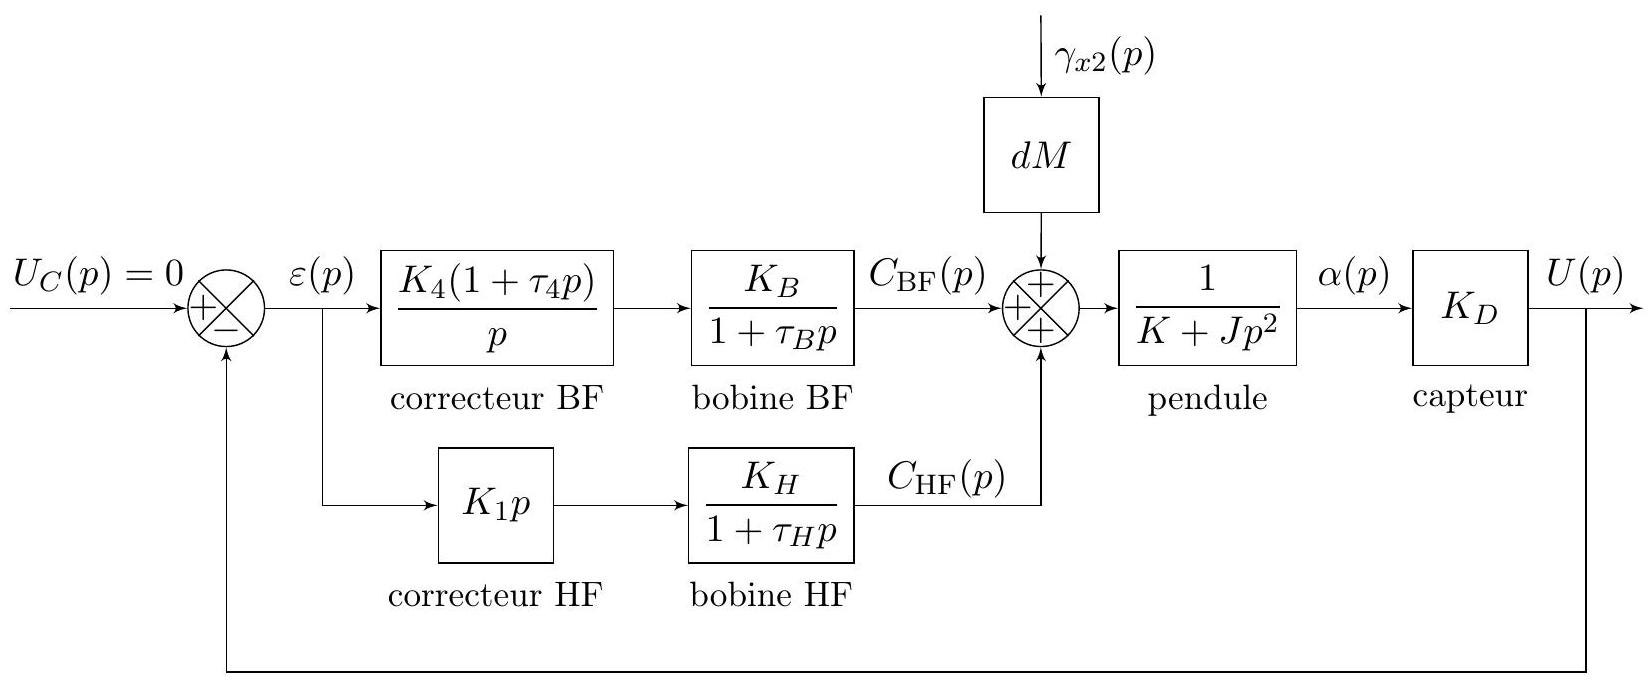
\includegraphics[width=.85\textwidth]{2024_04_26_3285cfc264024262add0g-19}
%\caption{\label{ccmp2023_fig_01}
\caption{Schéma-blocs de l'asservissement}
\end{figure}

%Grandeurs physiques intervenant dans l'asservissement

\begin{table}[!h]
\centering
\begin{tabular}{p{2cm}p{2cm}p{1cm}p{10cm}}
\hline
Grandeur physique & Transformée de Laplace  & Unité & Description \\
\hline
$u_{C}(t)$ & $U_{C}(p)$ & $\mathrm{V}$ & Tension consigne. Elle est toujours nulle car on souhaite que le pendule revienne à sa position d'équilibre.  \\
\hline
$u(t)$ & $U(p)$ & $\mathrm{V}$ & Tension en sortie du capteur, image du déplacement angulaire du pendule autour de sa position d'équilibre. \\
\hline
$\varepsilon(t)$ & $\varepsilon(p)$ & $\mathrm{V}$ & Écart entre la tension de consigne et la tension en sortie du capteur  \\
\hline
$\gamma_{x 2}(t)$ & $\gamma_{x 2}(p)$ & $\mathrm{m} \cdot \mathrm{s}^{-2}$ & Accélération du sol lors d'un séisme \\
\hline
$\Delta \alpha(t)$ & $\alpha(p)$ & $\mathrm{rad}$ & Déplacement angulaire du pendule autour de sa position d'équilibre \\
\hline
$C_{\mathrm{BF}}(t)$ & $C_{\mathrm{BF}}(p)$ & $\mathrm{N} \cdot \mathrm{m}$ & Moment généré par la bobine BF sur l'axe de rotation du pendule \\
\hline
$C_{\mathrm{HF}}(t)$ & $C_{\mathrm{HF}}(p)$ & $\mathrm{N} \cdot \mathrm{m}$ & Moment généré par la bobine HF sur l'axe de rotation du pendule \\
\hline
\end{tabular}
\caption{Grandeurs physiques intervenant dans l'asservissement}

\end{table}

\section*{Données numériques}
\begin{multicols}{3}
\begin{itemize}
  \item $K_{D}=1,48 \times 10^{5} \si{V} \cdot \mathrm{rad}^{-1}$
  \item $K_{H}=3 \times 10^{-8} \si{N} \cdot \mathrm{m} \cdot \mathrm{V}^{-1}$
  \item $\tau_{H}=0,001 \si{s}$
  \item $K_{B}=5 \times 10^{-8} \si{N} \cdot \mathrm{m} \cdot \mathrm{V}^{-1}$
  \item $\tau_{B}=0,1 \si{s}$
\end{itemize}
\end{multicols}




